\patternTwo

\subsection*{Context}

    Diagrams are an important form of representation, especially in technical disciplines. They are used for communication between people and for documentation. 
Such diagrams are usually precisely specified. 

In computer science, \ac{uml} diagrams  are widely used. There are specifications for \ac{uml}. Formats are defined for the data exchange of \ac{uml} models. 
Some software tools support code generation or reverse engineering.

In the first two semesters, it is mainly class diagrams that are taught.

Class diagrams primarily show the elements within classes and the relationships between classes as two-dimensional visual graphics.
    
\subsection*{Problem}

\begin{itshape}
Graphical representations of diagrams are not accessible to \ac{bvi} learners.
\end{itshape}

\subsection*{Solution}

\begin{sol}
Analyze which concepts are represented by the diagram and find a textual representation for them. 
Implicit information as expressed by the spatial arrangement of diagram elements can be made tangible with haptic interface devices.  
\end{sol}

Most software modeling tools use  a textual storage format. These formats are often not designed for humans but are used for data exchange. One example is \ac{xmi}\footnote{\url{https://www.omg.org/spec/XMI/}} for the exchange of \ac{uml} models. Model elements are represented textually as XML structures .

There are tools that use a simple textual representation that is easier for humans to read. UML4ALL, PlantUML and Mermaid are examples of such text based \ac{uml} tools.
These tools generate diagrams from the textual description for visual users. 
\ac{bvi} learners can have the textual description read aloud using text-to-speech, use screen readers or read on Braille lines.

A two-dimensional graphic is perceived by sighted people by “jumping” between the spatially arranged elements with the eye.
\ac{bvi} learners have sequential, one-dimensional access to the textual description. In order not to increase the cognitive load unnecessarily, information on relationships between elements should be provided near to the description of the elements.
The spatial arrangement of elements in a diagram often contains implicit information such as grouping or proximity of content. 
Such information can be made haptically accessible to \ac{bvi} learners. Examples include 2D Braille displays or structured surfaces (Swell Touch Paper, 3D printing).




\subsection*{Examples}
 
Listing \ref{lst:uml} is an example of a textual description following these recommendations and \ref{fig:class_diagram} shows the generated \ac{uml} class diagram. 


\begin{lstlisting}[label = lst:uml,  caption = {PlantUML source code}, basicstyle=\footnotesize]
@startuml
class Person {
  + firstname: String
  + surname: String
}
class Student {
  + matriculationNumber: int
  + degreeProgram: String
}
Person ^-- Student
class Lecturer {
  + title: String
  + department: String
}
Person ^-- Lecturer
class Book {
  + title: String
  + ISBN: String
}
Student "1" o-- "n" Book
@enduml
\end{lstlisting}

\begin{figure}[ht]
    \centering
    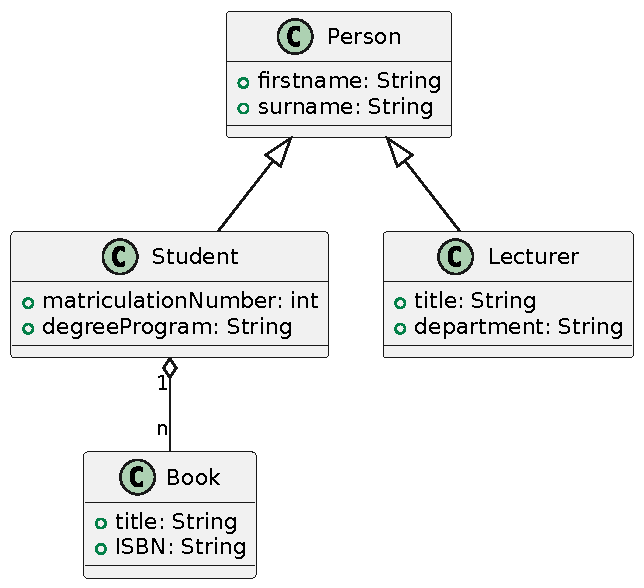
\includegraphics[width=.6\linewidth]{img/classDiagram.pdf}
    \caption{Generated \ac{uml} Class Diagram}
    \label{fig:class_diagram}
\end{figure}

\subsection*{Consequences}

% Benefits
\renewcommand{\labelenumi}{$+$}
\begin{enumerate}
\item Multi-modal accessibility is achieved by making textual explanations of diagrams accessible using assistive technology. 

\item Haptic devices can make information available that is contained in the spatial arrangement of elements in diagrams.

\item Textual descriptions of diagrams can be used in part to generate code. 
\end{enumerate}

% Liabilities
\renewcommand{\labelenumi}{$-$}
\begin{enumerate}
\item A new, purely text-based representation must be learned for the creation of teaching materials.

\item Changes and corrections are often more time-consuming, as the graphic representation must be re-rendered after changes are made.

\item Text-based exchange formats such as XMI are designed to be easily processed by software – but not primarily for human readability.
\end{enumerate} 
 
\subsection*{Related Work}

In \cite{doore2023} a \ac{mds} facilitates the perception of graphical information for \ac{bvi} students by integrating multiple sensory modalities: visual, auditory, and haptic. 
The system generates an auditory representation of diagrams by means of programmatically generated sine wave tones. Simultaneously, haptic feedback is delivered via a vibration motor, triggered when a user’s finger contacts specific x-y screen coordinates corresponding to points, lines, or curves. 

In \cite{king2007} the author present a project which makes  the content of UML diagrams accessible for \ac{bvi} students. In that project, a user interface for Windows was developed using the standard components of Microsoft Windows so that it is compatible with screen readers. This allows experienced users to use their usual screen reader. In addition, alternative interfaces such as spatial sound or a force feedback joystick are used to display spatial information on the diagram. 



In \cite{wildhaber2020} a solution is presented that allows visually impaired people easy access to class diagrams.
It utilizes existing accessibility tools of current mobile devices. A physically tactile grid is attached over a tablet so that a tactile navigation is possible.
By using Apple software, navigation can be carried out with the native VoiceOver solution, which is well known among  visually impaired people.
The authors developed a user interface which arranges classes in a grid.  Detailed information is displayed in a separate area, which can be navigated using the  VoiceOver system. 
In studies, the authors have compared their solution with the \ac{tml} PlantUML. Across several studies, the authors found that their solution is often better suited to new users, as it significantly lowers the learning curve compared to PlantUML.